%% arrowLength=10
%% linkWidth=3
%% input fy=50*node.pos
%% output fx=350
%% output fy=50*node.pos+50
%% MAX_FONT_SIZE=8
\begin{table}[H]
    \begin{center}
        \begin{tabular}{||l c c c||}
            \hline
            & 1        & 2        & 3 \\ [0.5ex]
            \hline
            velikost populacije               & 200      & 250      & 350      \\
            \hline
            največje število globokih vozlišč & 15       & 20       & 40       \\
            \hline
            največje število povezav          & 30       & 50       & 100      \\
            \hline
            največje število prečkanj         & 2        & 3        & 4        \\
            \hline
            delež mutiranih potomcev          & 10\%     & 10\%     & 10\%     \\
            \hline
            prispevek kompleksnosti           & -0.00001 & -0.00001 & -0.00001 \\
            \hline
            število generacij                 & 200      & 200      & 300      \\
            \hline
        \end{tabular}
    \end{center}
    \caption{Nabori inicializacijskih parametrov poganjanja na množici Car Evaluation.}
    \label{tab:param_car}
\end{table}

\subsection{Prvi nabor}\label{subsec:dodatek-car-prvi-nabor}
%%"/home/jure/CLionProjects/Neuroevolution/datasets/car/car.data" 200 15 30 2 true 0.1 100 true -0.00001 200 ACC
\begin{table}[H]
    \begin{center}
        \begin{tabular}{|| c | c c || c c ||}
            \hline
            \multirow{2}{*}{št. zagona} & \multicolumn{2}{c||}{točnost najboljšega agenta} & \multicolumn{2}{c||}{MCC najboljšega agenta} \\ \cline{2-5}
            & učna   & testna          & učna  & testna                  \\
            \hline
            1        & 71.7\% & 71.4\%          & 0.507 & 0.454                   \\
            \hline
            2        & 72.6\% & 73.4\%          & 0.477 & 0.486                   \\
            \hline
            3        & 74.0\% & \textbf{73.6\%} & 0.457 & 0.431                   \\
            \hline
            4        & 71.4\% & 71.0\%          & 0.496 & \textbf{0.487 (73.7\%)} \\
            \hline
            5        & 72.1\% & 70.7\%          & 0.483 & 0.403                   \\
            \hline
            $\sigma$ & 0.009  & 0.012           & 0.017 & 0.032                   \\
            \hline
        \end{tabular}
    \end{center}
    \caption{Rezultat prvega nabora parametrov.}
    \label{tab:car_result_1}
\end{table}

\begin{table}[H]
    \centering
    \begin{tabular}{||rccccc||}
        \hline
        razred       & unacceptable & acceptable & good & very good & vsota \\ \hline
        unacceptable & 354          & 0          & 9    & 0         & 363   \\ \hline
        acceptable   & 100          & 14         & 1    & 0         & 115   \\ \hline
        good         & 8            & 0          & 13   & 0         & 21    \\ \hline
        very good    & 10           & 1          & 8    & 0         & 19    \\ \hline
        vsota        & 472          & 15         & 31   & 0         & 518   \\ \hline
    \end{tabular}
    \caption{Matrika zmot najbolj točnega agenta prvega nabora. Agent ne more napovedati razreda \enquote{zelo dobro}.}
    \label{tab:car_acc_1}
\end{table}

\begin{table}[H]
    \centering
    \begin{tabular}{||rccccc||}
        \hline
        razred       & unacceptable & acceptable & good & very good & vsota \\ \hline
        unacceptable & 289          & 74         & 0    & 0         & 363   \\ \hline
        acceptable   & 22           & 93         & 0    & 0         & 115   \\ \hline
        good         & 0            & 21         & 0    & 0         & 21    \\ \hline
        very good    & 0            & 19         & 0    & 0         & 19    \\ \hline
        vsota        & 311          & 207        & 0    & 0         & 518   \\ \hline
    \end{tabular}
    \caption{Matrika zmot agenta z največjim MCC prvega nabora. Agent lahko napove samo razreda \enquote{nesprejemljivo} in \enquote{sprejemljivo}.}
    \label{tab:car_mcc_1}
\end{table}

\begin{figure}[H]
    \begin{center}
        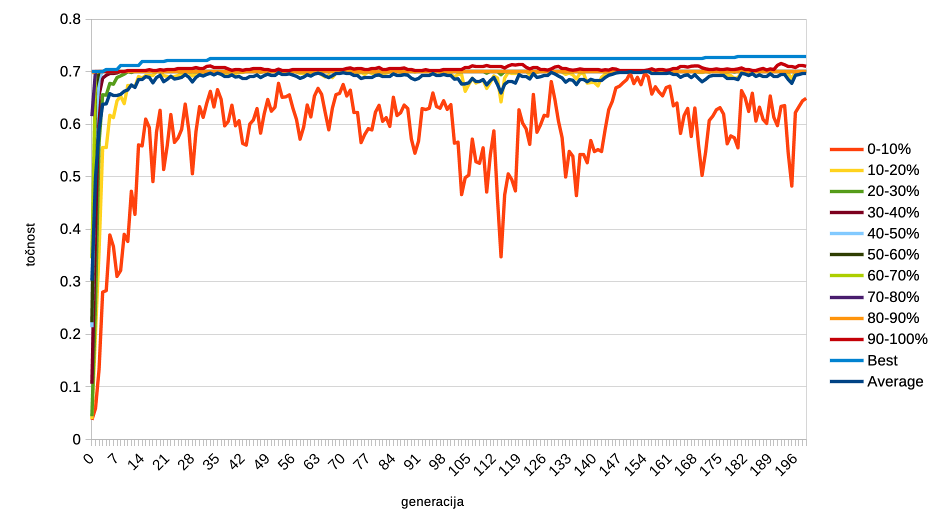
\includegraphics[width=13cm]{car/1/acc}
    \end{center}
    \caption{Graf točnosti populacije najboljšega agenta prvega nabora skozi generacije.}
    \label{fig:car_acc_1}
\end{figure}

\begin{figure}[H]
    \begin{center}
        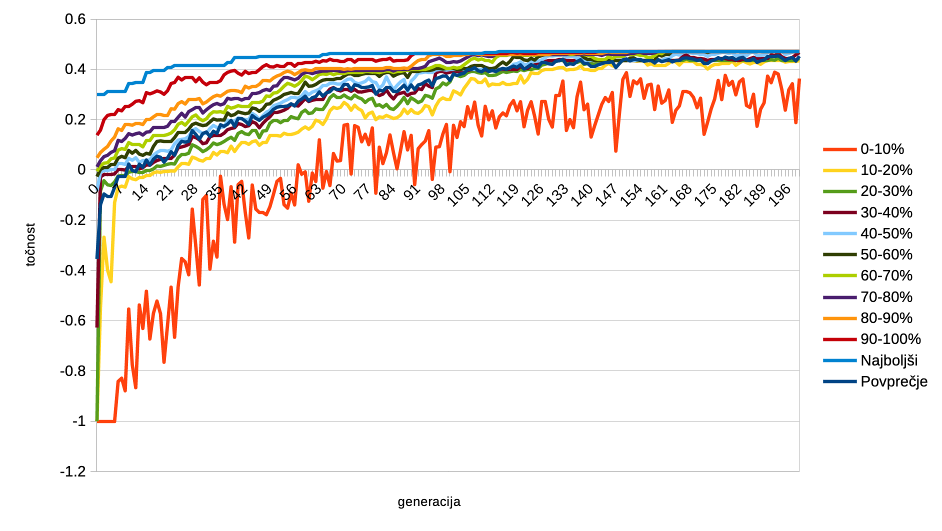
\includegraphics[width=13cm]{car/1/mcc}
    \end{center}
    \caption{Graf MCC populacije najboljšega agenta prvega nabora skozi generacije.}
    \label{fig:car_mcc_1}
\end{figure}

\begin{figure}[H]
    \begin{center}
        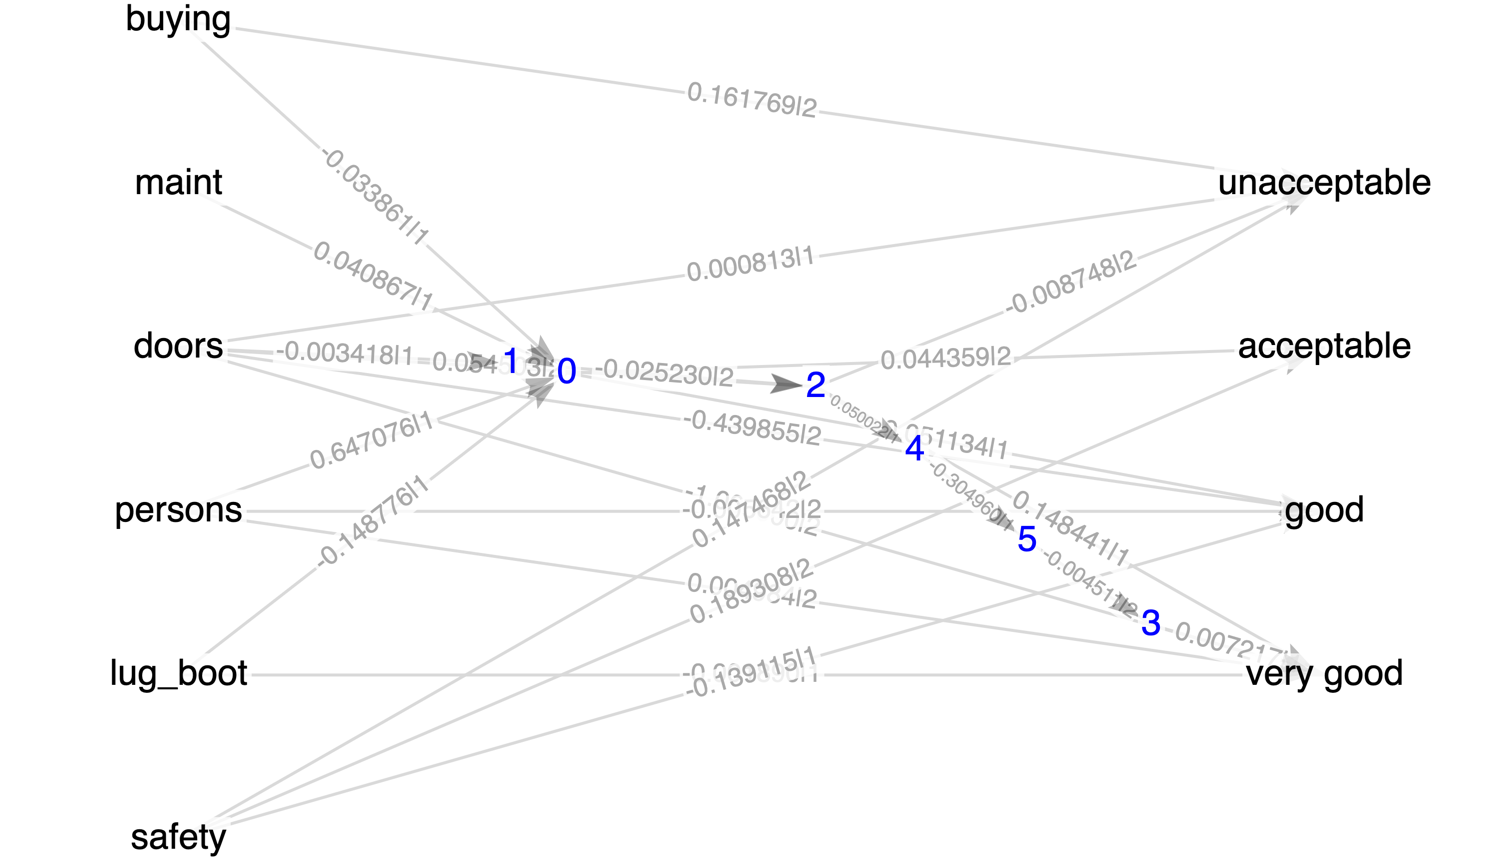
\includegraphics[width=13cm]{car/1/acc_g}
    \end{center}
    \caption{Vizualizacija najbolj točnega agenta prvega nabora. Vsebuje 10 povezav.}
    \label{fig:car_acc_1_g}
\end{figure}

\begin{figure}[H]
    \begin{center}
        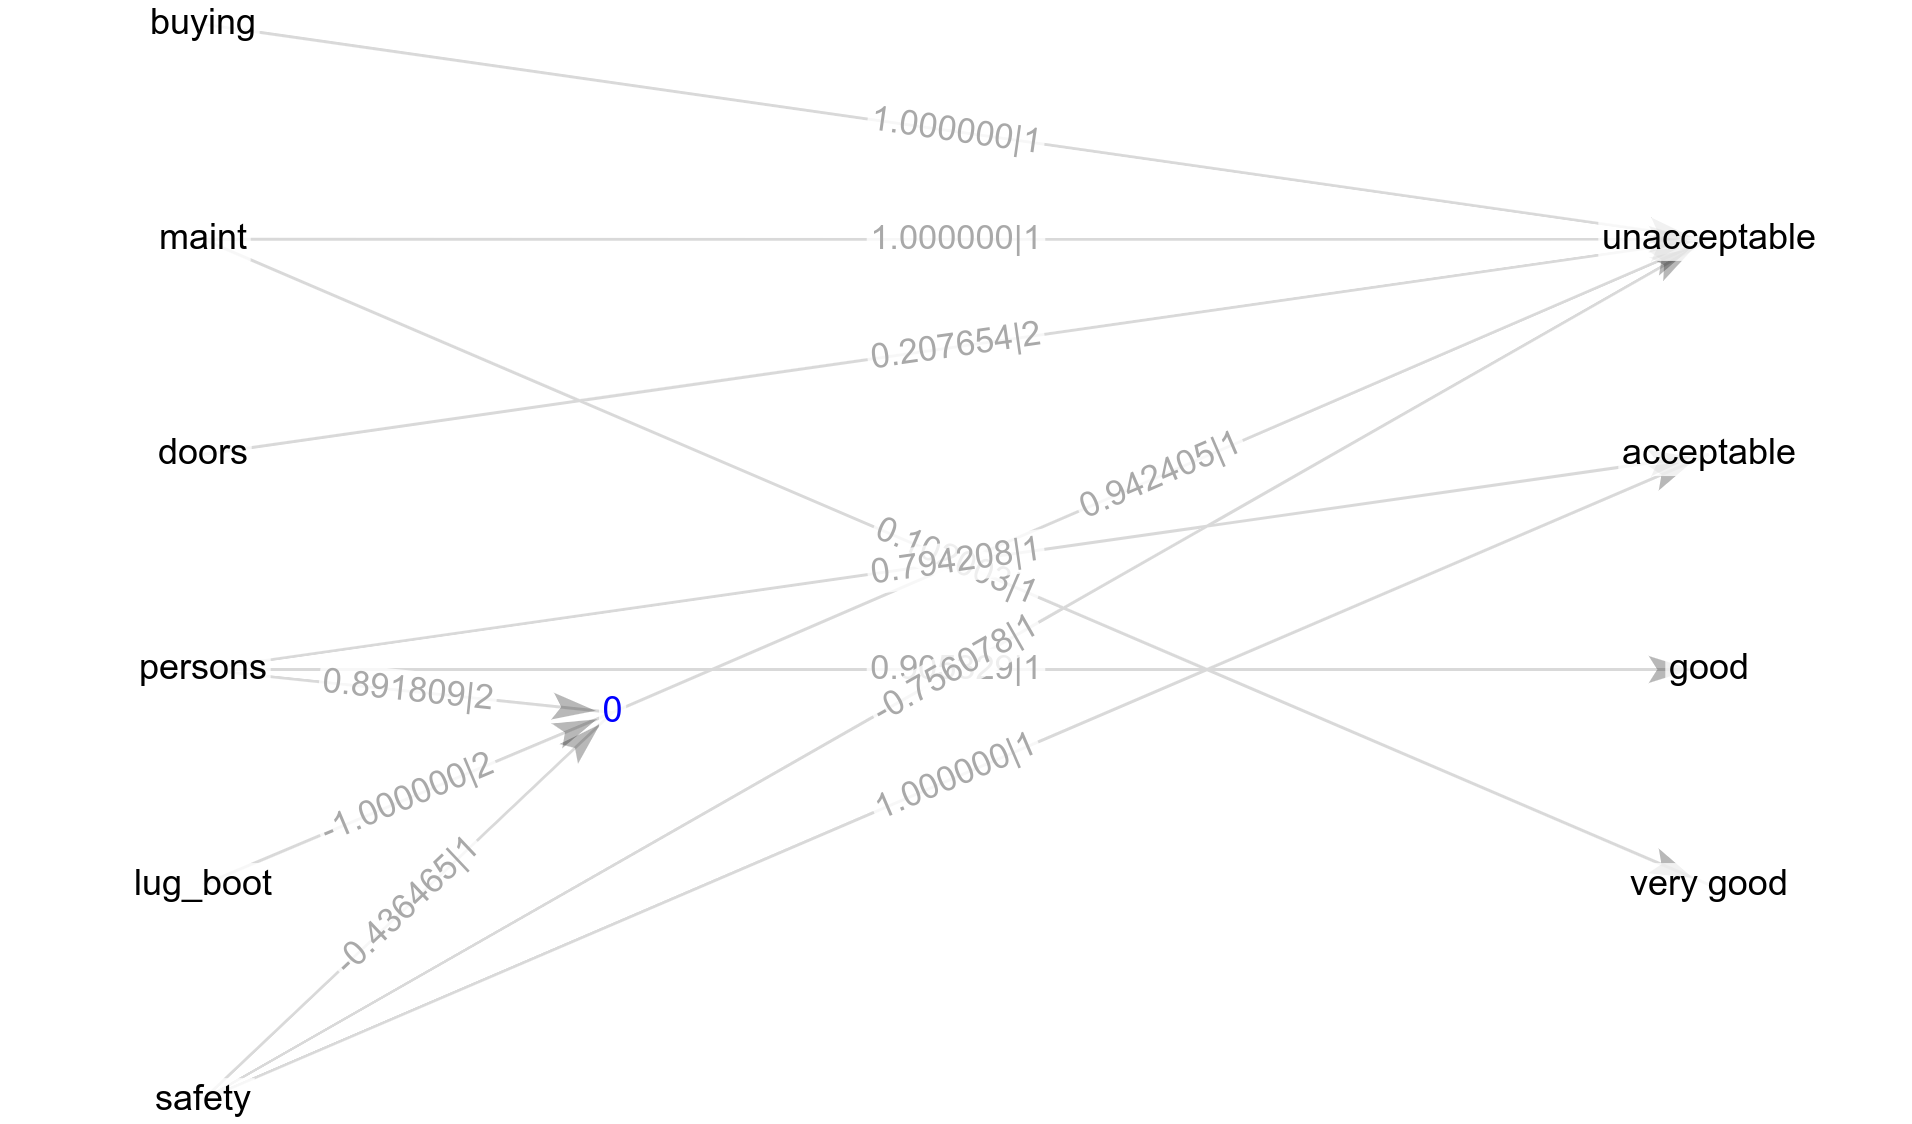
\includegraphics[width=13cm]{car/1/mcc_g}
    \end{center}
    \caption{Vizualizacija agenta z največjim MCC prvega nabora. Vsebuje 1 globoko vozlišče in 12 povezav.}
    \label{fig:car_mcc_1_g}
\end{figure}

\subsection{Drugi nabor}\label{subsec:dodatek-car-drugi-nabor}
%% 250 20 50 3 true 0.1 125 true -0.00001 200 ACC
\begin{table}[H]
    \begin{center}
        \begin{tabular}{|| c | c c || c c ||}
            \hline
            \multirow{2}{*}{št. zagona} & \multicolumn{2}{c||}{točnost najboljšega agenta} & \multicolumn{2}{c||}{MCC najboljšega agenta} \\ \cline{2-5}
            & učna   & testna          & učna  & testna                  \\
            \hline
            1        & 76.6\% & \textbf{74.3\%} & 0.502 & 0.470                   \\
            \hline
            2        & 74.9\% & 68.3\%          & 0.481 & 0.484                   \\
            \hline
            3        & 71.9\% & 72.0\%          & 0.485 & 0.493                   \\
            \hline
            4        & 72.3\% & 72.8\%          & 0.565 & \textbf{0.585 (75.9\%)} \\
            \hline
            5        & 72.3\% & 71.0\%          & 0.492 & 0.457                   \\
            \hline
            $\sigma$ & 0.018  & 0.02            & 0.031 & 0.045                   \\
            \hline
        \end{tabular}
    \end{center}
    \caption{Rezultat drugega nabora parametrov.}
    \label{tab:car_result_2}
\end{table}

\begin{table}[H]
    \centering
    \begin{tabular}{||rccccc||}
        \hline
        razred       & unacceptable & acceptable & good & very good & vsota \\ \hline
        unacceptable & 325          & 38         & 0    & 0         & 363   \\ \hline
        acceptable   & 55           & 60         & 0    & 0         & 115   \\ \hline
        good         & 0            & 21         & 0    & 0         & 21    \\ \hline
        very good    & 0            & 19         & 0    & 0         & 19    \\ \hline
        vsota        & 380          & 138        & 0    & 0         & 518   \\ \hline
    \end{tabular}
    \caption{Matrika zmot najbolj točnega agenta drugega nabora. Agent lahko napove samo razreda \enquote{nesprejemljivo} in \enquote{sprejemljivo}.}
    \label{tab:car_acc_2}
\end{table}

\begin{table}[H]
    \centering
    \begin{tabular}{||rccccc||}
        \hline
        razred       & unacceptable & acceptable & good & very good & vsota \\ \hline
        unacceptable & 271          & 67         & 0    & 25        & 363   \\ \hline
        acceptable   & 7            & 107        & 0    & 1         & 115   \\ \hline
        good         & 0            & 9          & 0    & 12        & 21    \\ \hline
        very good    & 0            & 4          & 0    & 15        & 19    \\ \hline
        vsota        & 278          & 187        & 0    & 53        & 518   \\ \hline
    \end{tabular}
    \caption{Matrika zmot agenta z največjim MCC drugega nabora. Agent ne more napovedati razreda \enquote{dobro}.}
    \label{tab:car_mcc_2}
\end{table}

\begin{figure}[H]
    \begin{center}
        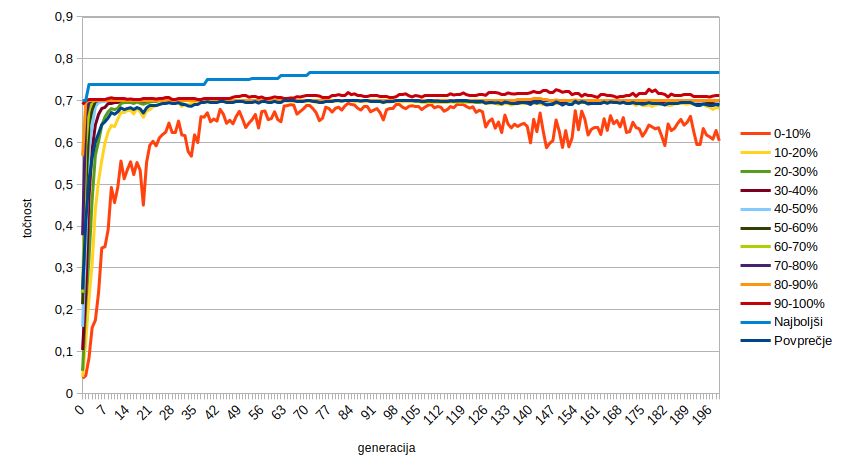
\includegraphics[width=13cm]{car/2/acc}
    \end{center}
    \caption{Graf točnosti populacije najboljšega agenta drugega nabora skozi generacije.}
    \label{fig:car_acc_2}
\end{figure}

\begin{figure}[H]
    \begin{center}
        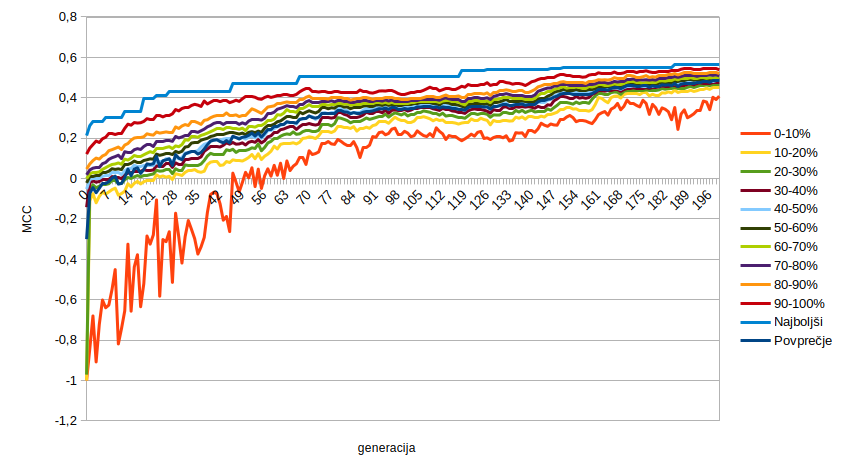
\includegraphics[width=13cm]{car/2/mcc}
    \end{center}
    \caption{Graf MCC populacije najboljšega agenta drugega nabora skozi generacije.}
    \label{fig:car_mcc_2}
\end{figure}

\begin{figure}[H]
    \begin{center}
        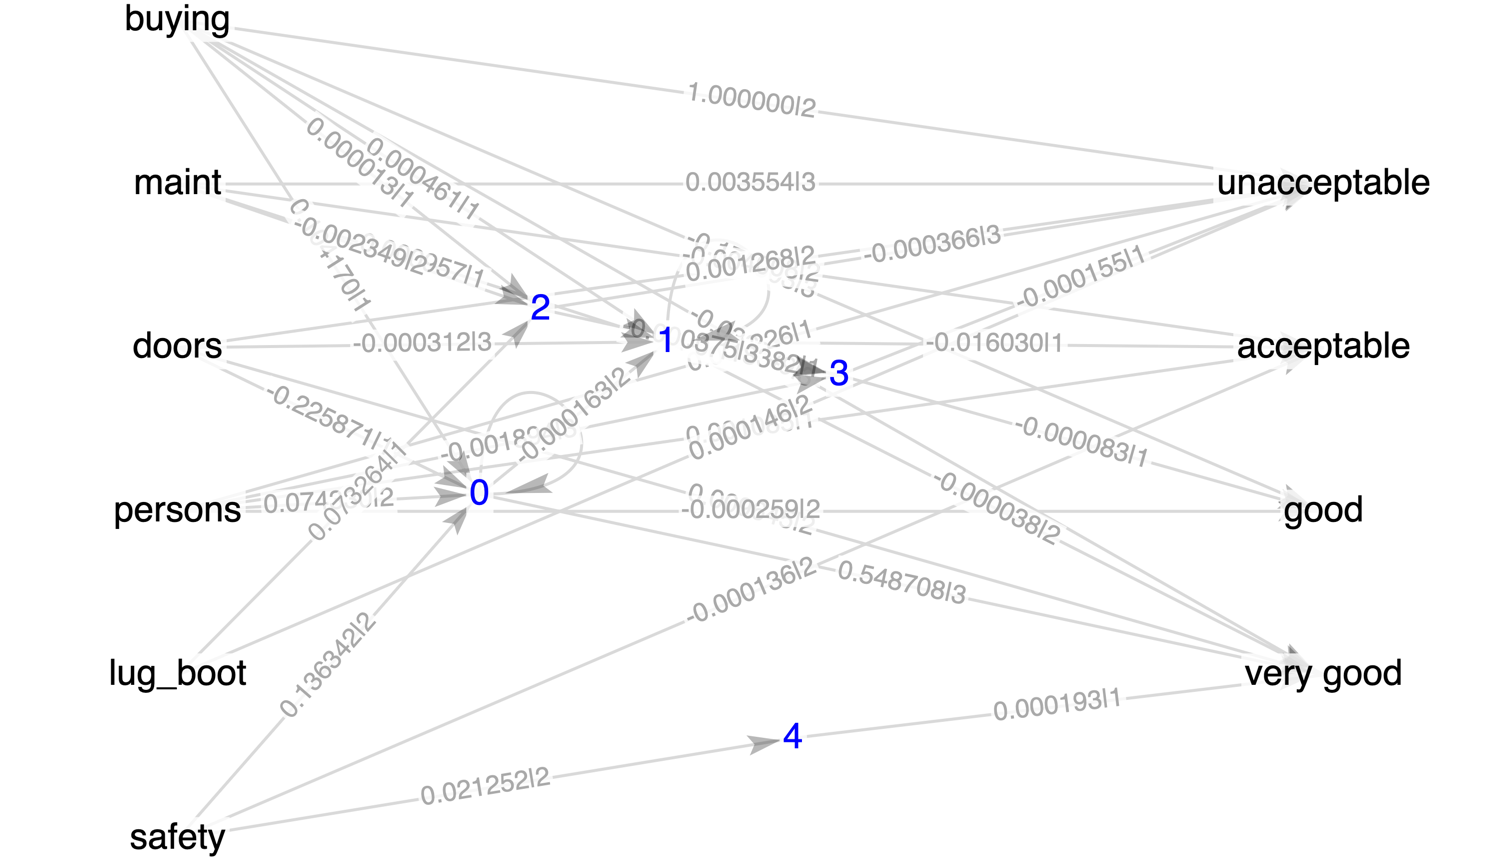
\includegraphics[width=13cm]{car/2/acc_g}
    \end{center}
    \caption{Vizualizacija najbolj točnega agenta drugega nabora. Vsebuje 1 globoko vozlišče in 16 povezav.}
    \label{fig:car_acc_2_g}
\end{figure}

\begin{figure}[H]
    \begin{center}
        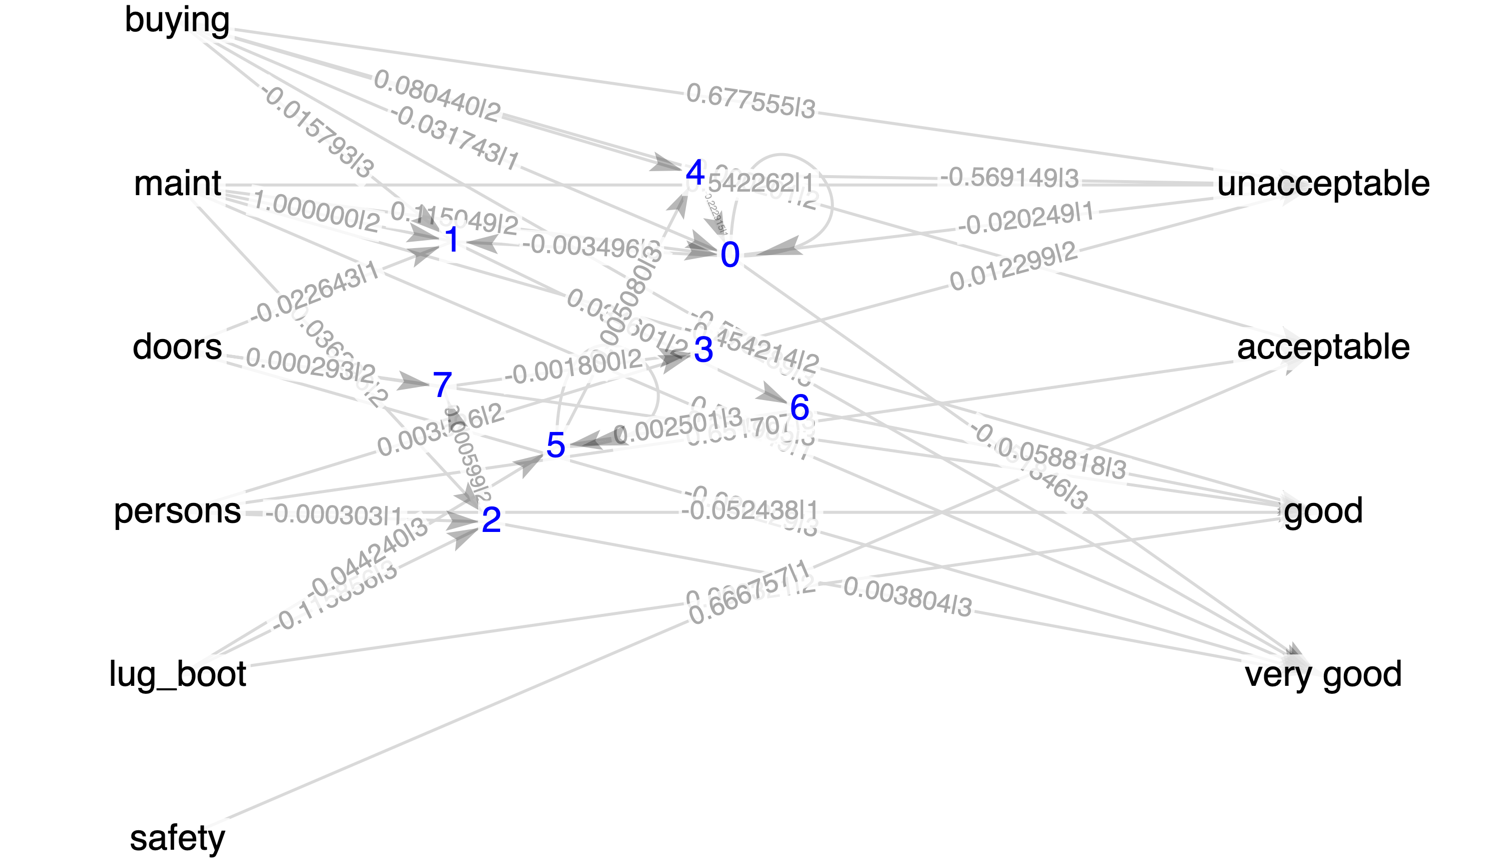
\includegraphics[width=13cm]{car/2/mcc_g}
    \end{center}
    \caption{Vizualizacija agenta z največjim MCC drugega nabora. Vsebuje 13 povezav.}
    \label{fig:car_mcc_2_g}
\end{figure}

\subsection{Tretji nabor}\label{subsec:dodatek-car-tretji-nabor}
%% 350 40 100 4 true 0.1 175 true -0.00001 300 ACC
\begin{table}[H]
    \begin{center}
        \begin{tabular}{|| c | c c || c c ||}
            \hline
            \multirow{2}{*}{št. zagona} & \multicolumn{2}{c||}{točnost najboljšega agenta} & \multicolumn{2}{c||}{MCC najboljšega agenta} \\ \cline{2-5}
            & učna   & testna          & učna  & testna                  \\
            \hline
            1        & 73.6\% & \textbf{73.6\%} & 0.510 & 0.498                   \\
            \hline
            2        & 73.1\% & 71.2\%          & 0.486 & 0.502                   \\
            \hline
            3        & 72.4\% & 70.8\%          & 0.493 & 0.462                   \\
            \hline
            4        & 73.5\% & 72.0\%          & 0.468 & 0.467                   \\
            \hline
            5        & 72.7\% & 72.8\%          & 0.516 & \textbf{0.539 (73.7\%)} \\
            \hline
            $\sigma$ & 0.005  & 0.010           & 0.017 & 0.028                   \\
            \hline
        \end{tabular}
    \end{center}
    \caption{Rezultat tretjega nabora parametrov.}
    \label{tab:car_result_3}
\end{table}

\begin{table}[H]
    \centering
    \begin{tabular}{||rccccc||}
        \hline
        razred       & unacceptable & acceptable & good & very good & vsota \\ \hline
        unacceptable & 325          & 38         & 0    & 0         & 363   \\ \hline
        acceptable   & 59           & 56         & 0    & 0         & 115   \\ \hline
        good         & 4            & 17         & 0    & 0         & 21    \\ \hline
        very good    & 0            & 19         & 0    & 0         & 19    \\ \hline
        vsota        & 388          & 130        & 0    & 0         & 518   \\ \hline
    \end{tabular}
    \caption{Matrika zmot najbolj točnega agenta tretjega nabora. Agent lahko napove samo razreda \enquote{nesprejemljivo} in \enquote{sprejemljivo}.}
    \label{tab:car_acc_3}
\end{table}

\begin{table}[H]
    \centering
    \begin{tabular}{||rccccc||}
        \hline
        razred       & unacceptable & acceptable & good & very good & vsota \\ \hline
        unacceptable & 270          & 66         & 0    & 27        & 363   \\ \hline
        acceptable   & 10           & 103        & 0    & 2         & 115   \\ \hline
        good         & 0            & 10         & 0    & 11        & 21    \\ \hline
        very good    & 0            & 10         & 0    & 9         & 19    \\ \hline
        vsota        & 280          & 189        & 0    & 49        & 518   \\ \hline
    \end{tabular}
    \caption{Matrika zmot agenta z največjim MCC tretjega nabora. Agent ne more napovedati razreda \enquote{dobro}.}
    \label{tab:car_mcc_3}
\end{table}

\begin{figure}[H]
    \begin{center}
        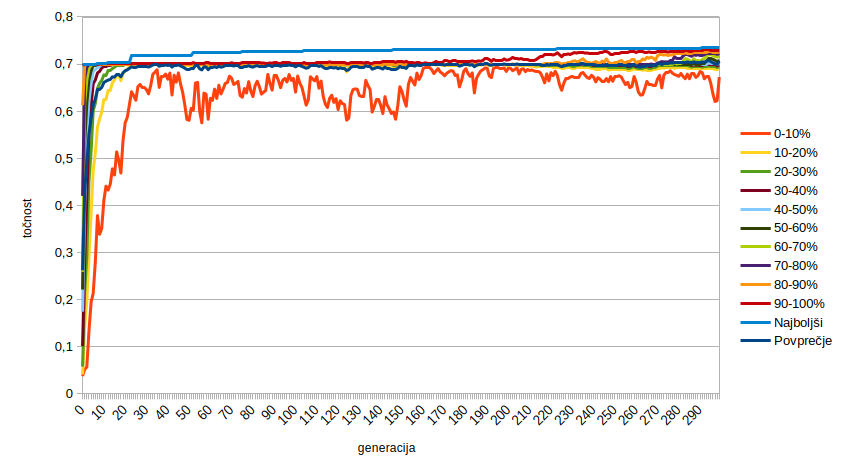
\includegraphics[width=13cm]{car/3/acc}
    \end{center}
    \caption{Graf točnosti populacije najboljšega agenta tretjega nabora skozi generacije.}
    \label{fig:car_acc_3}
\end{figure}

\begin{figure}[H]
    \begin{center}
        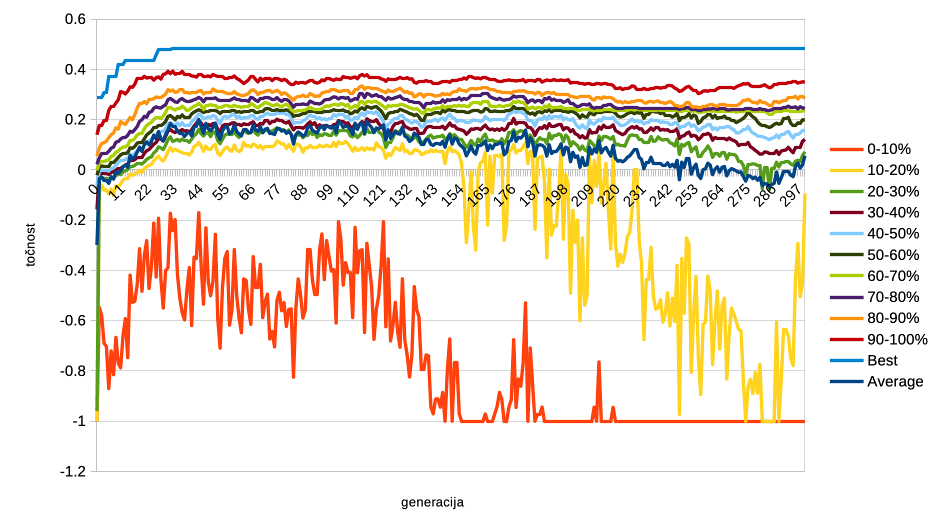
\includegraphics[width=13cm]{car/3/mcc}
    \end{center}
    \caption{Graf MCC populacije najboljšega agenta tretjega nabora skozi generacije.}
    \label{fig:car_mcc_3}
\end{figure}

\begin{figure}[H]
    \begin{center}
        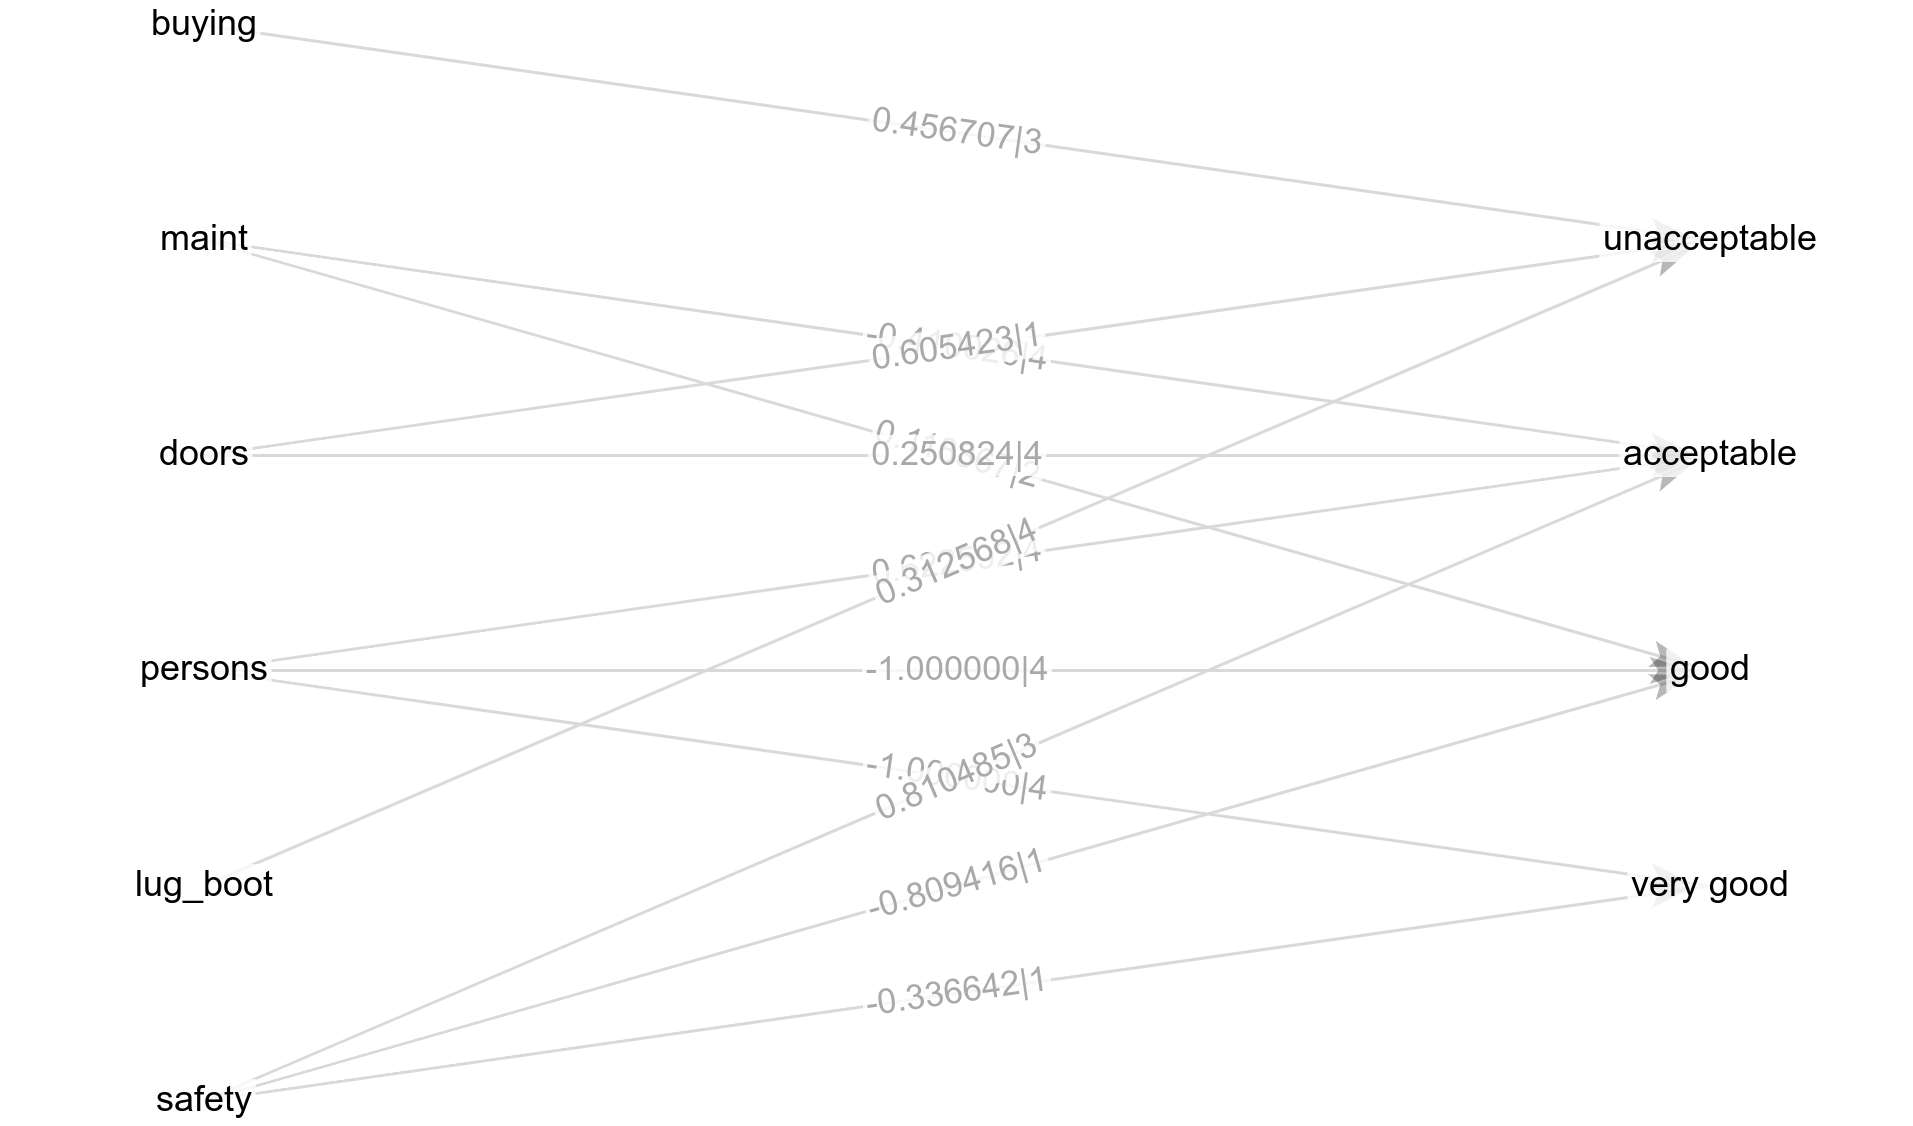
\includegraphics[width=13cm]{car/3/acc_g}
    \end{center}
    \caption{Vizualizacija najbolj točnega agenta tretjega nabora. Vsebuje 12 povezav.}
    \label{fig:car_acc_3_g}
\end{figure}

\begin{figure}[H]
    \begin{center}
        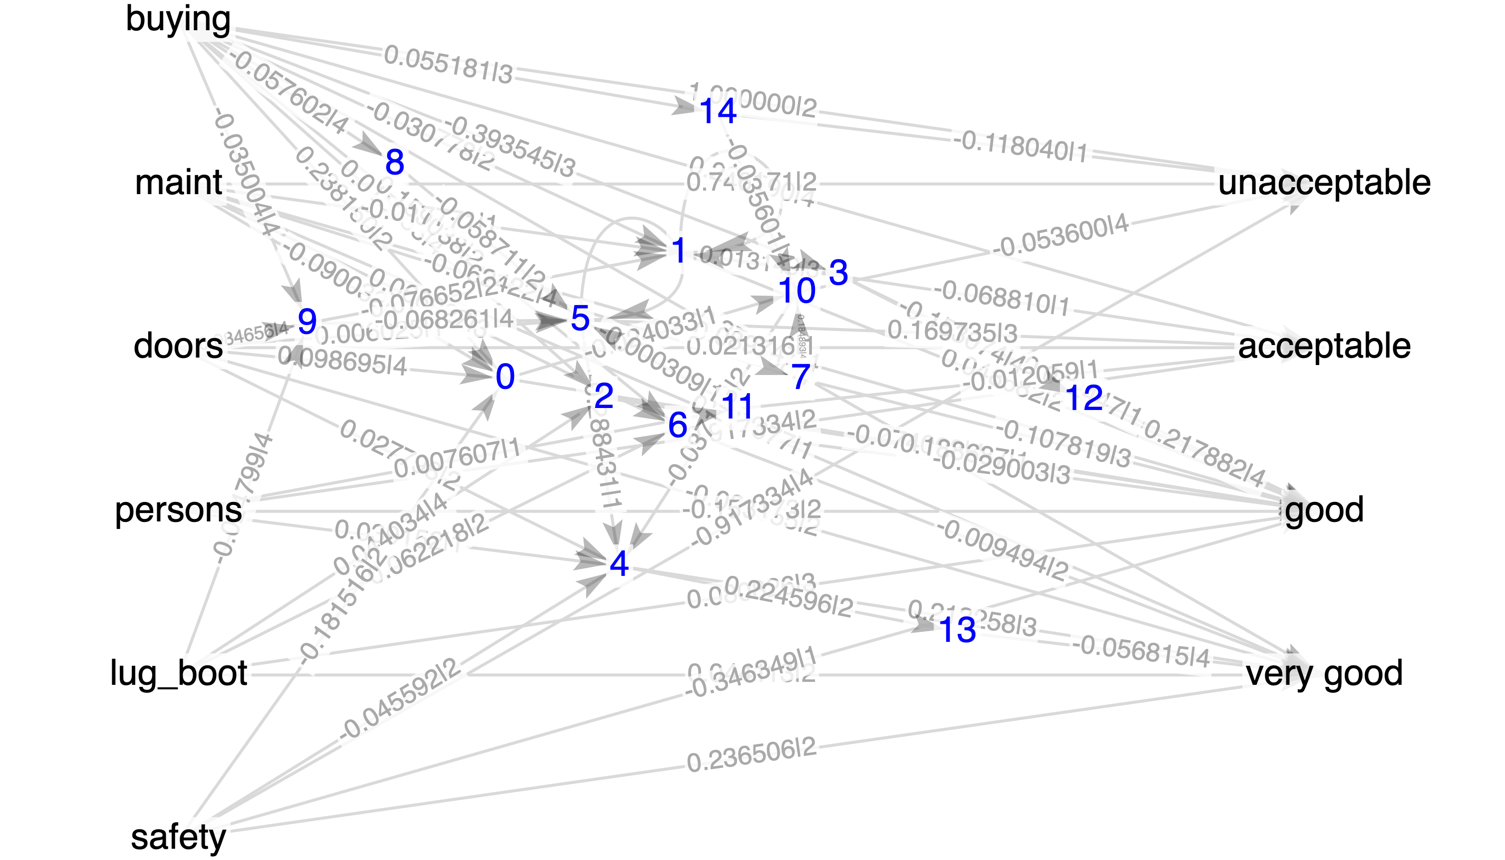
\includegraphics[width=13cm]{car/3/mcc_g}
    \end{center}
    \caption{Vizualizacija agenta z največjim MCC drugega nabora. Vsebuje 13 povezav.}
    \label{fig:car_mcc_3_g}
\end{figure}